
\documentclass[template=tabling,81pt,headonall]{azmoon}
\usepackage{xepersian}
\usepackage{amsfonts}
\usepackage{graphicx}
\usepackage{svg}
\svgpath{ {./images/} }
\graphicspath{ {./images/} }
\settextfont{Yas}
\setdigitfont{A Iranian Sans}
\usepackage{fontawesome5}

\printanswers
    \teacher{محمد صالح علی اکبری}
    \teachertitle{دبیر}
    \city{گناباد}
    \schooltitle{متوسطه دوره اول}
    \school{مقداد}
    \grade{هشتم}
    \branch{۱}
    \topic{ریاضی}
    \examdate{دی ۱۴۰۲}
    \answertime{۹۰ دقیقه}
    \begin{document}
	\begin{questions}
		\nointerlineskip%
		\vskip-\baselineskip
		\question[1]{%
حاصل عبارت‌های زیر را حساب کنید.
    \begin{LTR}
        \begin{parts}[2]\part{$ 300 - 20 + 30 = $}
\part{$5 -80 + 10 + 80 = $}
\end{parts}
\end{LTR}
        
    }\question[1]{%
حاصل عبارت‌های زیر را حساب کنید.
    \begin{LTR}
        \begin{parts}[2]\part{$2 \times (3)  = $}
\part{$4 \times (-7) = $}
\end{parts}
\end{LTR}
        
    }\question[2]{%
حاصل تقسیم‌های زیر را محاسبه کنید.
    \begin{parts}[4]\part{ 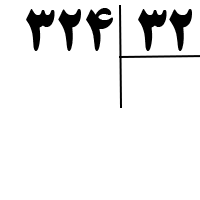
\includegraphics[scale = 0.18]{تقسیم5}}
\part{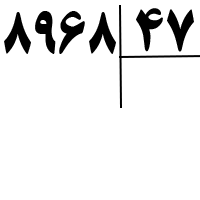
\includegraphics[scale = 0.18]{تقسیم8}}
\end{parts}
‌
\\‌
\\‌
\\
    }\question[4]{%
حاصل جمع و تفریق‌های زیر را محاسبه کنید.
    \begin{LTR}
        \begin{parts}[1]\part{$\dfrac{2}{3}+\dfrac{2}{7} = $}
\part{$-\dfrac{4}{3}+\dfrac{1}{9} = $}
\part{$4.2-5.1 = $}
\part{$6.2 - 5.7 = $}
\end{parts}
\end{LTR}
        
    }\question[2]{%
حاصل ضرب و تقسیم‌های زیر را محاسبه کنید.
    \begin{LTR}
        \begin{parts}[1]\part{$+\dfrac{4}{4}\times\dfrac{1}{8} = $}
\part{$\dfrac{7}{2}\times\dfrac{6}{5} = $}
\end{parts}
\end{LTR}
        
    }\question[3]{%
شمارنده‌های اعداد زیر را بدست آورید.
    \begin{parts}[2]\part{$24$}
\part{$10$}
\part{$4$}
\end{parts}

    }\question[2]{%
ک.م.م. اعداد زیر را بدست آورید.
    \begin{parts}[2]\part{$12 , 6$}
\part{$12 , 6$}
\end{parts}

    }\question[2]{%
ب.م.م. اعداد زیر را بدست آورید.
    \begin{parts}[2]\part{$45 , 15$}
\part{$27 , 36$}
\end{parts}

    }\question[1.5]{%
مجموع اعداد زیر را محاسبه کنید. \\1+2+3+...+54+55+56 = }\question[1.5]{%
محیط و مساحت شکل زیر را محاسبه کنید. \\ 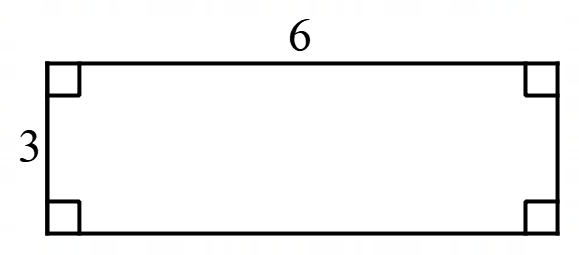
\includegraphics[scale = 1]{مستطیل}}\end{questions}
    \end{document}
    